\documentclass[12pt]{beamer}
\usepackage{mathtools}
\useoutertheme{infolines}
\usetheme{default}
\usefonttheme{serif}
%\usefonttheme{structuresmallcapsserif}
\hypersetup{colorlinks=true,linkcolor=blue}
\setbeamertemplate{navigation symbols}{}
\author{Mittereder, \textit{et. al.}}
\definecolor{darkgreen}{rgb}{0,.5,0}
\setlength{\parskip}{.1in}

\begin{document}

\begin{frame}[c]{} % Justin

\begin{center}
\Large
Exploring the Impact of Social Network Density\\and Agent Openness on Societal Polarization

\footnotesize
\vspace{.3in}
CSS 2021 --- Santa Fe, New Mexico (sorta)\\
\vspace{.1in}
Justin Mittereder, Robert S.~W.~Carroll, Brandon Frulla, Stephen Davies\\
\scriptsize
\smallskip
Dept of Computer Science\\
University of Mary Washington\\
Fredericksburg, Virginia, USA\\
\end{center}

\end{frame}

\begin{frame}[c]{Defining polarization} % Justin

\large

\centering
``America is becoming increasingly polarized..."

\vspace{-.2in}
\begin{figure}
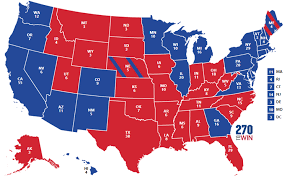
\includegraphics[width=0.35\textwidth]{usa.png}
\end{figure}
\pause
\vspace{-.2in}
What does this actually mean?
\vspace{-.15in}
\pause

\small
\begin{itemize}
\itemsep.1em
\item People's views becoming more \textit{extreme}?
\pause
\item People becoming more \textit{stubborn}? (less willing to reconsider views)
\pause
\item People only associating with like-minded others?
\end{itemize}

\end{frame}

\begin{frame}[c]{Proxy \#1: Assortativity coefficient} % Justin

{\tiny \color{red} Justin TODO: This is an old slide from a previous talk, in which I talk
about nominal (binary/categorical; i.e., red and blue) opinions instead of
continuous opinions. You can reuse any of this, or just throw it away, and
replace with content about aggregate assortativity over continuous opinions.}

A graph's \textit{(nominal) assortativity coefficient} is the fraction of
edges that are between same-valued nodes, compared to what we would expect if
the edges were dispersed at random.

\begin{itemize}
\itemsep.1em
\item 1 --- ``perfect" assortative mixing (all edges are between nodes of the
same value)
\item 0 --- no assortative mixing (node values have no impact on whether nodes
will connect)
\item a negative number --- (nodes tend to connect to nodes of
\textit{different} values)

\end{itemize}

\end{frame}

\begin{frame}[c]{Assortativity coefficient} % Justin
\centering
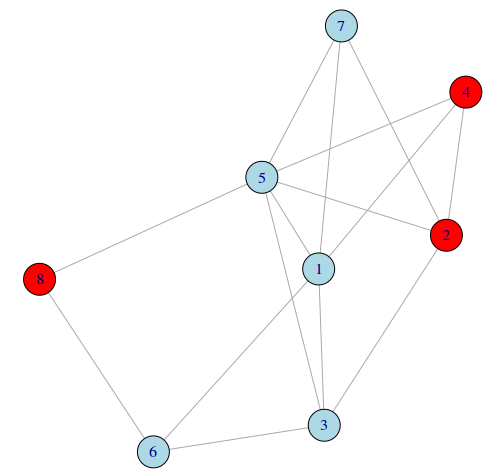
\includegraphics[width=0.4\textwidth]{assortativityGraph.png}

7 blue--blue edges and 1 red--red edge\\
7 red--blue edges\\
Assortativity coefficient: 0.111

\end{frame}


\begin{frame}[c]{Proxy \#2: Issue Alignment} % Stephen

We define \textbf{Issue Alignment} (IA) as the tendency for people who agree on
one issue to also agree on other (unrelated) issues.

{\tiny \color{red} 
Stephen TODO:

\begin{itemize}
\itemsep.1em
\item Illustrative list of typical left vs. right positions
\item Ask: in your experience, does this hold true?
\end{itemize}
}

\end{frame}

\begin{frame}[c]{One possible explanation for IA} % Stephen

{\tiny \color{red} 
Stephen TODO:

Perhaps there is some deep underlying principle to people's ideologies that
connects seemingly unconnected issues. (Maybe for some deep reason it actually
makes sense that people who are pro-life are also pro-gun, and anti-tax, and
anti-vacc.)
}

\end{frame}

\begin{frame}[c]{Another possible explanation for IA} % Stephen

{\tiny \color{red} 
Stephen TODO:

Perhaps a small number of popular media outlets each articulates a number of
opinions on various issues. The people who listen to them are naturally
influenced to each of these different opinion values, and thus become ``issue
aligned."
}

\end{frame}

\begin{frame}[c]{A third possible explanation for IA} % Stephen

We define \textbf{Cross-Issue Influence} (CI2) as the effect that a person's
social contact can have on one of their opinions based on their agreement (or
disagreement) on a different issue.

{\tiny \color{red} 
Stephen TODO:

We wish there was more justification in the social psych lit for this, but we
have to fall back on (1) homophily and (2) common sense.

Big idea: even without any underlying ideological connection between issues,
and even without media influence, IA will naturally develop solely due to CI2.
In other words, CI2 is sufficient for IA. (Wide reaching implications on how we
interpret the causes of the polarization phenomenon, and what societal changes
might be necessary to reduce it.)
}

\end{frame}

\begin{frame}[c]{CI2 in detail}  % Justin

\end{frame}

\begin{frame}[c]{}

\begin{center}
\Large
Exploring the Impact of Social Network Density\\and Agent Openness on Societal Polarization

\footnotesize
\vspace{.3in}
CSS 2021 --- Santa Fe, New Mexico (sorta)\\
\vspace{.1in}
Justin Mittereder, Robert S.~W.~Carroll, Brandon Frulla, Stephen Davies\\
\smallskip
\scriptsize
Dept of Computer Science\\
University of Mary Washington\\
Fredericksburg, Virginia, USA\\
\end{center}

\end{frame}
\end{document}
